\documentclass{scrartcl}
\usepackage[utf8]{inputenc}
\usepackage{graphicx}
\usepackage{geometry}
\usepackage{titling}

% Configuration
\graphicspath{ {img/} }
\geometry{a4paper}

\renewcommand\partheadstartvskip{\clearpage\null\vfil}
\renewcommand\partheadmidvskip{\par\nobreak\vskip 20pt\thispagestyle{empty}}
\renewcommand\partheadendvskip{\vfil\clearpage}
\renewcommand\raggedpart{\centering}


% Title
\title{Yet Another Stupid Compiler}
\author{
    Louis Solofrizzo\\
    \texttt{louis@ne02ptzero.me}\\
    \\
    42 Staff\\
    \texttt{staff@42.fr}
}

\pretitle{%
    \begin{center}
    \LARGE
    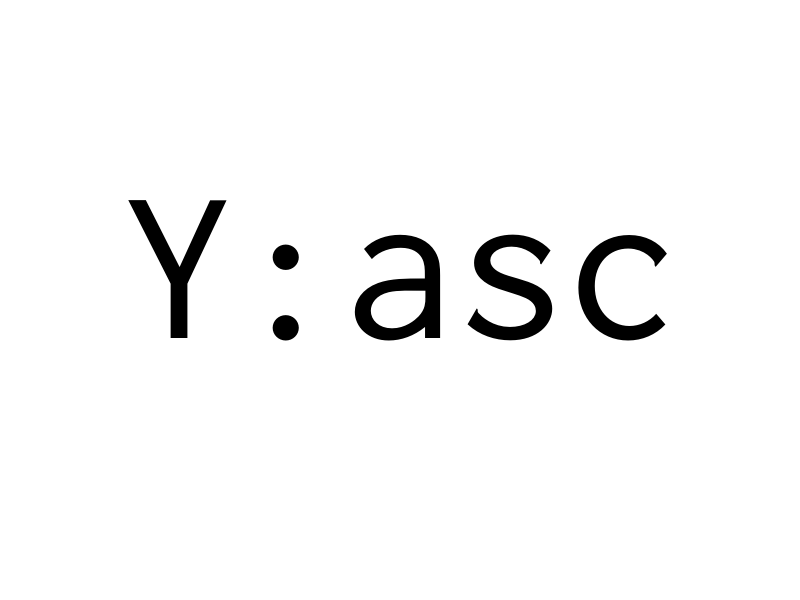
\includegraphics[scale=0.1, height=7cm]{logo}\\[\bigskipamount]
}

\posttitle{%
    \end{center}
}


% Actual document
\begin{document}

\begin{titlingpage}
    \maketitle
\end{titlingpage}


    \tableofcontents{}
    \newpage

\part{Introduction}
\part{The Y Language}
    \section{Getting Started}
    \section{Types, Operators and Expressions}
        \subsection{Variable names}
        \subsection{Namespaces}
        \subsection{Data types and Sizes}
        \subsection{Constants}
        \subsection{Declarations}
        \subsection{Arithmetic Operators}
        \subsection{Type Conversions}
        \subsection{Assignement Operators and Expressions}
        \subsection{Conditionnal Expressions}
        \subsection{Precedence and Order of Evaluation}
    \section{Control Flow}
        \subsection{If-Else}
        \subsection{Else-If}
        \subsection{Loops - While}
        \subsection{Loops - For}
        \subsection{Loops - Do-While}
        \subsection{Break and Continue}
    \section{Functions and Program Structure}
        \subsection{Basics}
        \subsection{External Variables}
        \subsection{Scope Rules}
        \subsection{Header Files}
        \subsection{Static Variables}
        \subsection{Recursion}
        \subsection{Preprocessor}
    \section{Pointers and Arrays}
        \subsection{Pointers and Addresses}
        \subsection{Pointers and Function Arguments}
        \subsection{Pointers and Arrays}
        \subsection{Address Arithmetic}
        \subsection{The \_\_heap argument}
        \subsection{Command-line Arguments}
    \section{Structures}
        \subsection{Basics}
        \subsection{Structures and Functions}
        \subsection{Array of Structures}
        \subsection{Pointer to Structures}
        \subsection{Packing}
    \section{Standard Library}
        \subsection{Input and Output}
        \subsection{Memory Control}
        \subsection{System Calls}
    \section{Format}
        \subsection{Comments}
        \subsection{Unicode}
        \subsection{Inline definitions}
\part{The ASC Language}
    \section{Getting Started}
    \section{Definitions}
    \section{Accessors}
        \subsection{Basics}
        \subsection{Special Accessors}
        \subsection{Constants}
    \section{Registers}
        \subsection{Infinite Registers}
        \subsection{Define a Register}
    \section{Memory}
        \subsection{Virtual Memory}
        \subsection{Paging}
        \subsection{On-Disk memory}
        \subsection{Cache}
    \section{Arithmetic}
        \subsection{Basics}
        \subsection{Comparisons}
        \subsection{Bit-Fields}
    \section{Calls}
        \subsection{Functions}
        \subsection{System Calls}
    \section{Format}
        \subsection{Comments}
        \subsection{Instructions}


\end{document}
